\documentclass[tikz, border=10pt]{standalone}
\usepackage{tikz}
\usetikzlibrary{shapes.geometric, arrows.meta, positioning, shadows, mindmap, trees}

\begin{document}
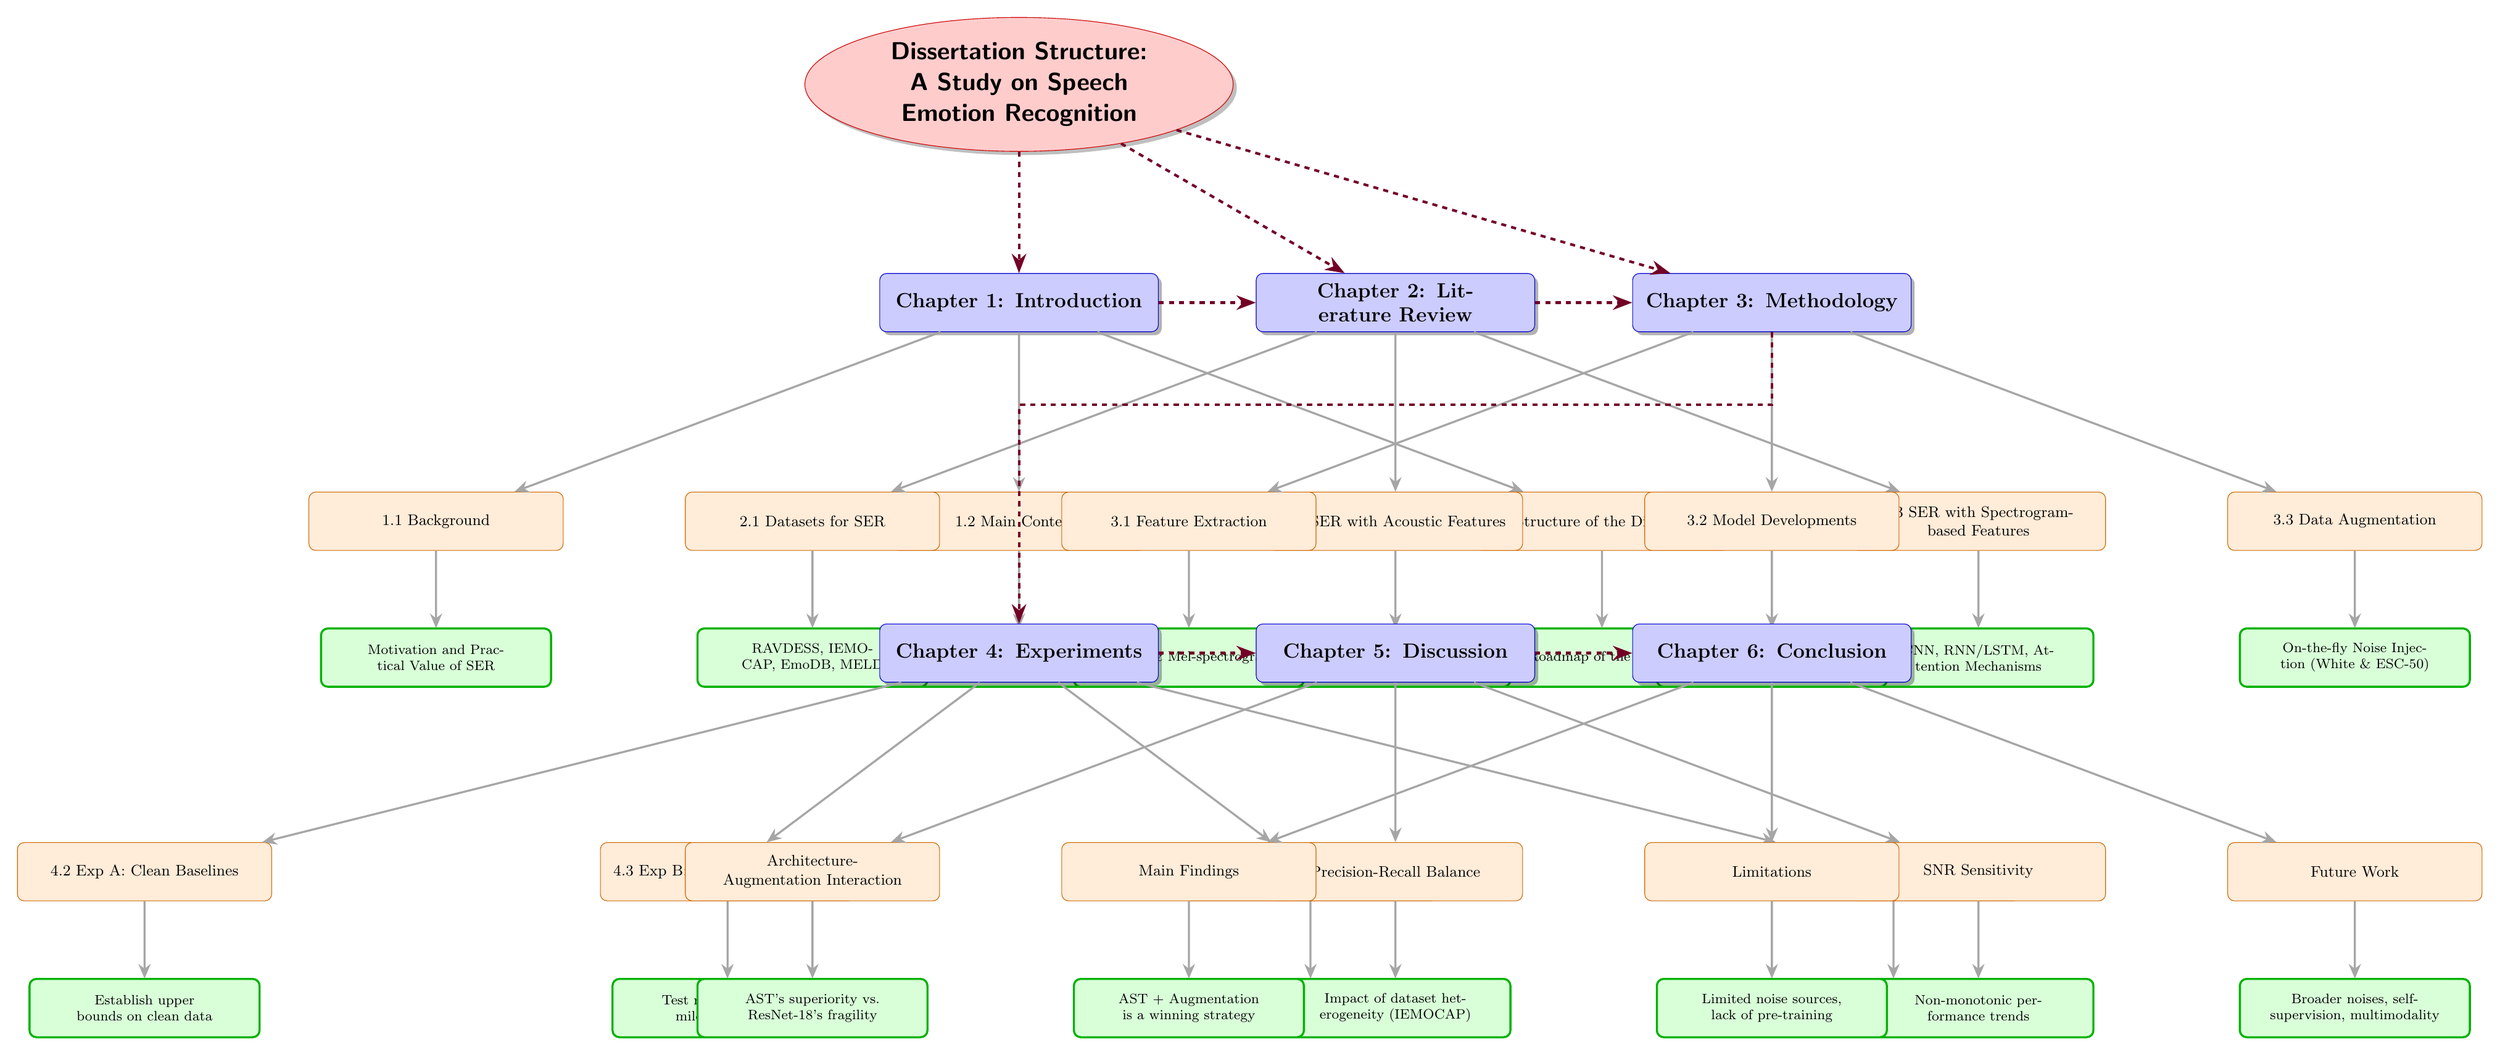
\begin{tikzpicture}[
    % Level 1: Chapters
    level 1/.style={
        rectangle, rounded corners, draw=blue!80!black, fill=blue!20,
        text width=5.5cm, minimum height=1.2cm, align=center,
        drop shadow={shadow xshift=2pt, shadow yshift=-2pt, fill=black, opacity=0.3},
        font=\large\bfseries,
        sibling distance=12cm, % Distance between chapters
        level distance=4.5cm     % Distance from title to chapters
    },
    % Level 2: Sections
    level 2/.style={
        rectangle, rounded corners, draw=orange!80!black, fill=orange!15,
        text width=5cm, align=center,
        font=\small,
        growth parent anchor=south,
        parent anchor=south,
        sibling distance=2mm, % Vertical distance between sections
        level distance=2.2cm   % Distance from chapter to sections
    },
    % Level 3: Sub-sections
    level 3/.style={
        rectangle, rounded corners, draw=green!70!black, fill=green!15,
        text width=4.5cm, align=center,
        font=\footnotesize,
        growth parent anchor=south,
        sibling distance=1mm,
        level distance=2cm
    },
    % Main Title
    title/.style={
        ellipse, draw=red!80!black, fill=red!20,
        text width=6cm, minimum height=1.5cm, align=center,
        font=\Large\bfseries\sffamily,
        drop shadow
    },
    % Edge styles
    edge from parent/.style={
        draw=gray!70, -{Stealth[length=3mm, width=2.5mm]}, very thick
    },
    % Connector line style
    connector/.style={
        draw=purple!60!black, -{Stealth[length=4mm, width=3mm]}, line width=1.5pt, dashed
    }
]

% Main Title Node
\node[title] (title) {Dissertation Structure: \\ A Study on Speech Emotion Recognition};

% Chapter Nodes (Level 1)
\node[level 1, below=2.5cm of title] (ch1) {Chapter 1: Introduction}
    child {node[level 2] {1.1 Background}
        child {node[level 3] {Motivation and Practical Value of SER}}
    }
    child {node[level 2] {1.2 Main Contents}
        child {node[level 3] {Objectives and Framework Overview}}
    }
    child {node[level 2] {1.3 Structure of the Dissertation}
        child {node[level 3] {Roadmap of the Thesis}}
    };

\node[level 1, right=2cm of ch1] (ch2) {Chapter 2: Literature Review}
    child {node[level 2] {2.1 Datasets for SER}
        child {node[level 3] {RAVDESS, IEMOCAP, EmoDB, MELD}}
    }
    child {node[level 2] {2.2 SER with Acoustic Features}
        child {node[level 3] {Prosodic, Spectral, Voice-Quality Features}}
    }
    child {node[level 2] {2.3 SER with Spectrogram-based Features}
        child {node[level 3] {CNN, RNN/LSTM, Attention Mechanisms}}
    };

\node[level 1, right=2cm of ch2] (ch3) {Chapter 3: Methodology}
    child {node[level 2] {3.1 Feature Extraction}
        child {node[level 3] {MFCC \& Mel-spectrogram}}
    }
    child {node[level 2] {3.2 Model Developments}
        child {node[level 3] {MLP, Shallow CNN, ResNet-18, AST}}
    }
    child {node[level 2] {3.3 Data Augmentation}
        child {node[level 3] {On-the-fly Noise Injection (White \& ESC-50)}}
    };

\node[level 1, below=6cm of ch1] (ch4) {Chapter 4: Experiments}
    child {node[level 2] {4.2 Exp A: Clean Baselines}
        child {node[level 3] {Establish upper bounds on clean data}}
    }
    child {node[level 2] {4.3 Exp B: White-Noise Training}
        child {node[level 3] {Test robustness with mild white noise}}
    }
    child {node[level 2] {4.4 Exp C: ESC-50 Multi-SNR}
        child {node[level 3] {Evaluate with realistic environmental noise}}
    }
    child {node[level 2] {4.5 Exp D: SNR Ablation}
        child {node[level 3] {Analyze performance across different SNRs}}
    };

\node[level 1, below=6cm of ch2] (ch5) {Chapter 5: Discussion}
    child {node[level 2] {Architecture-Augmentation Interaction}
        child {node[level 3] {AST's superiority vs. ResNet-18's fragility}}
    }
    child {node[level 2] {Precision-Recall Balance}
        child {node[level 3] {Impact of dataset heterogeneity (IEMOCAP)}}
    }
    child {node[level 2] {SNR Sensitivity}
        child {node[level 3] {Non-monotonic performance trends}}
    };

\node[level 1, below=6cm of ch3] (ch6) {Chapter 6: Conclusion}
    child {node[level 2] {Main Findings}
        child {node[level 3] {AST + Augmentation is a winning strategy}}
    }
    child {node[level 2] {Limitations}
        child {node[level 3] {Limited noise sources, lack of pre-training}}
    }
    child {node[level 2] {Future Work}
        child {node[level 3] {Broader noises, self-supervision, multimodality}}
    };

% Draw connecting arrows between chapters
\draw[connector] (ch1) -- (ch2);
\draw[connector] (ch2) -- (ch3);
\draw[connector] (ch3.south) -- ++(0, -1.5) -| (ch4.north);
\draw[connector] (ch4) -- (ch5);
\draw[connector] (ch5) -- (ch6);

% Connect Title to the first row of chapters
\draw[connector] (title) -- (ch1);
\draw[connector] (title) -- (ch2);
\draw[connector] (title) -- (ch3);

\end{tikzpicture}
\end{document}